% ---
% school: "college"
% level: "8eme"
% section: null
% chapter: "التناظر المركزي"
% source: "Axiomaths"
% title: "مثلث قائم ومنتصف الوتر"
% country: "Tunisie"
% year: 2026
% professor: "Axiomaths"
% difficulty: "Facile"
% points: null
% tags: ["symetrie-centrale", "triangle-rectangle", "rectangle", "perimetre"]
% ---
% Exercice 4/15 de la série 8ème « التناظر المركزي » (statement + \axsol + solution). Compiler avec XeLaTeX + axiomath.sty (+ axiomaths-logo.png).
\documentclass[12pt,a4paper]{article}
\usepackage[level=8b,color=15803D]{axiomath}
\usetikzlibrary{arrows.meta}
\newcommand{\cm}{\,\mathrm{cm}}
\axsetup{title={التناظر المركزي}, corrige}

\begin{document}

\begin{corr}[title={مثلث قائم ومنتصف الوتر}, stars=2, source={Axiomaths}]
$ABC$ مثلث قائم الزاوية في $A$ حيث $AB=3\cm$ و $AC=4\cm$ و $BC=5\cm$. $O$ منتصف $[BC]$.
\begin{center}
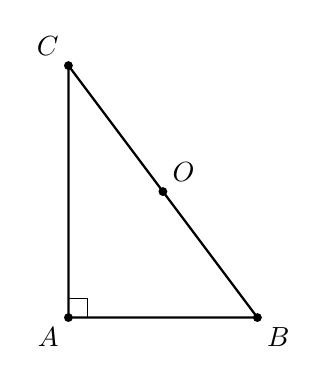
\begin{tikzpicture}[scale=0.8]
  \draw[thick] (0,0)--(3,0)--(0,4)--cycle;
  \draw (0,0.3)--(0.3,0.3)--(0.3,0);
  \fill (0,0) circle (2pt) node[below left] {$A$};
  \fill (3,0) circle (2pt) node[below right] {$B$};
  \fill (0,4) circle (2pt) node[above left] {$C$};
  \fill (1.5,2) circle (2pt) node[above right] {$O$};
\end{tikzpicture}
\end{center}
\begin{enumerate}
  \item ما هما مناظرا $B$ و $C$ بالنسبة إلى $O$ ؟
  \item ابنِ $A'$ مناظرة $A$ بالنسبة إلى $O$. ما هو مناظر المثلث $ABC$ ؟ احسب محيطه.
  \item بين أن $ABA'C$ مستطيل، ثم احسب $AA'$.
\end{enumerate}
\axsol
\begin{enumerate}[itemsep=14pt]
  \item $O$ منتصف $[BC]$ ، إذن مناظرة $B$ هي $C$ ومناظرة $C$ هي $B$.
  \item التناظر المركزي يحوّل $A$ إلى $A'$ و $B$ إلى $C$ و $C$ إلى $B$ ، فمناظر $ABC$ هو المثلث $A'CB$.
  \begin{prop}[الحفاظ على الأطوال والزوايا]
  التناظر المركزي يحفظ \ib{الأطوال} و \ib{قيس الزوايا}.
  \end{prop}
  إذن $A'C=AB=3\cm$ و $A'B=AC=4\cm$ و $CB=BC=5\cm$ ، ومحيط $A'CB$ هو :
  \[3+4+5=12\cm\]
  وهو نفس محيط $ABC$. الزاوية في $A'$ قائمة لأنها مناظرة الزاوية القائمة في $A$.
  \begin{center}
  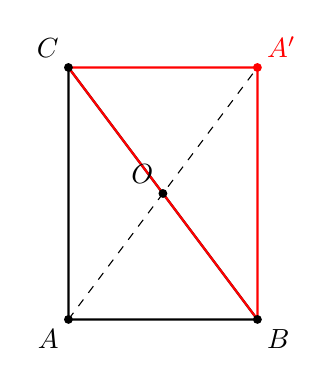
\begin{tikzpicture}[scale=0.8]
    \draw[thick] (0,0)--(3,0)--(0,4)--cycle;
    \draw[thick,red] (3,4)--(0,4)--(3,0)--cycle;
    \draw[dashed] (0,0)--(3,4);
    \fill (0,0) circle (2pt) node[below left] {$A$};
    \fill (3,0) circle (2pt) node[below right] {$B$};
    \fill (0,4) circle (2pt) node[above left] {$C$};
    \fill (1.5,2) circle (2pt) node[above left] {$O$};
    \fill[red] (3,4) circle (2pt) node[above right] {$A'$};
  \end{tikzpicture}
  \end{center}
  \item \begin{prop}[قطرا متوازي الأضلاع]
  رباعي قطراه يتقاطعان في منتصفهما هو متوازي أضلاع.
  \end{prop}
  القطران $[AA']$ و $[BC]$ للرباعي $ABA'C$ لهما نفس المنتصف $O$ ، إذن $ABA'C$ متوازي أضلاع.
  زاويته في $A$ قائمة، فهو \ib{مستطيل}. وقطرا المستطيل متقايسان :
  \[AA'=BC=5\cm\]
\end{enumerate}
\end{corr}

\end{document}
